%Discovery Notes(up to 4 pages, this is approx. 3000 words) Discovery notes report biologically interesting discoveries using computational techniques.

%Application Notes (up to 2 pages; this is approx. 1300 words or 1000 words plus one figure) Applications Notes are short descriptions of novel software or new algorithm implementations, databases and network services (web servers, and interfaces). 

\documentclass{bioinfo}
\copyrightyear{}
\pubyear{}
%\firstpage{}
\usepackage{amsmath, amssymb}
\usepackage{natbib}
\usepackage{tikz}
\usepackage{pgfplots}
\pgfplotsset{width=7cm,compat=1.5.1} 
\pgfplotsset{width=7cm} 
\usepackage[
   colorlinks=true, linkcolor=red, 
   citecolor=blue, urlcolor=blue
 ]{hyperref} 

\usepackage{txfonts}
%  $$$: 
%\usepackage[subscriptcorrection,txsy]{mtpro}
%\usepackage[mtphrb]{mtpams}
%\usepackage[mtpcal, mtpfrak]{mtpb}
%
\newcommand{\bA}{\textsf{\textit{A}}}
\newcommand{\bC}{\textsf{\textit{C}}}
\newcommand{\bG}{\textsf{\textit{G}}}
\newcommand{\bT}{\textsf{\textit{T}}}
%
%
% -----------------------------------------------------------
%
\begin{document}
\title[AID hotspots]{Constitution Analysis} 
 \author[I. T. Silva~\textit{et~al}]{%
     Israel T. Silva\,$^{1,3,}$\footnote{to
  whom correspondence should be addressed}\ , 
  and
       Rafael A. Rosales\,$^2$
  }

 \address{$^{1}$Laboratory of Molecular Immunology, The Rockefeller 
     University, 1230 York Avenue, New York, NY 10065\\
     $^{2}$Departamento de Computa\c{c}\~ao e Matem\'atica,
     Universidade de S\~ao Paulo. Av. Bandeirantes, 3900,
     Ribeir\~ao Preto,  CEP 14049-901, SP, Brazil%\\
%     $^{3}$National Institute of Science and Technology in Stem Cell
%     and Cell Therapy and Center for Cell Based Therapy. Rua Cat\~ao
%     Roxo, 2501, Ribeir\~ao Preto, CEP 14051-140, SP, Brazil
}

\history{Received on XXXXX; revised on XXXXX; accepted on XXXXX}
\editor{Associate Editor: XXXXXXX}

\maketitle
\begin{abstract}
  \section{Motivation:}
  \section{Results:} 
  \href{https://github.com/someone/rich}{\texttt{https://github.com/someone/rich}}.
  \section{Contact:}
  \href{mailto:someone@somewhere.world}{\tt someone@somewhere.world}%,
\end{abstract}

\section{Introduction}
The genome is targeted by a sophisticated and highly coordinated series of molecular events.  Among these events, aberrant DNA methylation patterns in human malignancy \cite{pmid23326238}, somatic retrotransposition in human cancers \cite{pmid22745252}, AID-dependent chromosomal translocations (Klein, 2011) and HIV integration (Cohn, 2014), which arrives throughout DNA, are not randomly distributed but instead associated with chromosomal regions and contributes to disrupt the integrity of the genome and human disease.

As result, these regions represents a genomic context in which are associate with multiple underlying mechanisms. The motif-based sequence analysis is the starting point to aim potential binding site of cis-regulatory elements associated. Nevertheless, the inherent low signal/noise ratio in sequence-based motif discovery is a limitation to detect a nucleic acid sequence pattern that has some biological significance. Moreover, these events may recognise a structural feature, rather than a specific sequence motif.

Others approaches were introduced to detect functional regions using methods for computing sequence complexities \cite{pmid24533097,pmid21317142}. In these methods, the complexity is measured by the entropy which evaluates the randomness of DNA sequence. In particular, topological entropy has been applied to compute the complexity of introns, exons and promoter regions. Due to the finite sample and high-dimensionality problems, efforts aimed to overcome these problems are put forward \cite{pmid21317142}.\footnote{its: I would prefer to leave entropy out unless we have a really good point we want to make}


Our work has some intersection whit the computation of `enrichment $p$-values' considered in  GO analysis. We may include the references \cite{HSL}, \cite{RPTP} (just one!) or any other if you know a better alternative. We may like to mention the paper by \cite{BM} because it also considers a test for enrichment (although it is restricted to ChiP-seq peaks, and somehow different).

However, how exactly the pattern nucleotide composition could influence the selection of target site selection are not well understood. To further characterize at a genome-wide scale these regions, we introduce a new method to provide a quantitative measure of the differential spectra of $k$-mers (DNA 'words' of length $k$) inside target DNA.


\section{Method}
Let $\mathcal A = \{\sf A, C, G, T\}$ and $\mathcal S \in \mathcal A^\ell$, be a given specific string of length $\ell\geq 1$. %\footnote{according to wikipedia an $\ell$-mer of a string is any possible substring of size $\ell$ of that string; clearly not what we want --I stick to string!}
In what follows, we describe a method to study the profile of $\mathcal S$ along a region of interest such as those defined by viral insertion or retrotranslocation hotspots. This provides the means to asses the significance of a differently distributed profiles along two functionally defined regions. We specialise to viral insertion hotspots as described by~\cite{IRAMM}, but the scope is clearly not restricted to this particular application. 

Let $h = \{h_1, \ldots, h_n\}$ bet a set of viral insertion hotspots, namely a set of DNA segments characterized by having a substantially high density of viral insertion events. Let $w$ be the length of the longest of such segments. The segments $h_1, \ldots, h_n$ are aligned with respect to their central base and then extended at both ends to have length $w$. Next, consider the partition of resulting set of segments into $k$ evenly spaced bins of length $\ell = w/k$. Denote by $h_{ij}$, $1 \leq j \leq k$, the $j$th bin of the $i$th segment. Consider now the set $r= \{r_1, \ldots, r_n\}$ of segments of width $w$ that are either at the left or at the right of any one segment in $h$. Likewise, let $r_{ij}$, $1\leq i \leq n$, $1 \leq j \leq k$, be the matrix formed by bins of length $\ell$ that result by partitioning  the elements of $r$. For any $j = 1, \ldots, k-1$ and $i = 1, \ldots, n$, let $\xi_{ij}$ and $\eta_{ij}$ be the following Bernoulli random variables
\begin{align*}
   &\xi_{ij} = %\mathbb 1_{\{\mathcal S \in h_{ij}\}} =
    \begin{cases}
     1, &\text{if } \mathcal S \in h_{ij} \text{ and } \mathcal S 
     \notin h_{i,j+1}\\
     1, &\text{if } \mathcal S \in h_{ij} \text{ and } \mathcal S 
     \in h_{i,j+1}\\
     0, &\text{otherwhise}
    \end{cases},\\
   &\eta_{ij} = %\mathbb 1_{\{\mathcal S \in h_{ij}\}} =
    \begin{cases}
     1, &\text{if } \mathcal S \in r_{ij} \text{ and } \mathcal S 
     \notin r_{i,j+1}\\
     1, &\text{if } \mathcal S \in r_{ij} \text{ and } \mathcal S 
     \in r_{i,j+1}\\
     0, &\text{otherwhise}
    \end{cases}.
\end{align*}
Set $\xi_{ik}  = 1$ if $\mathcal S \notin h_{i,k-1}$ and $\mathcal S \in h_{i,k-1}$, and $\xi_{ik} = 0$ otherwhise. Similarly define $\eta_{ik}$ by using the information in $r_{ik}$. Finaly, let
\[
   \xi_j = \sum_{i=1}^n \xi_{ij}, \qquad 
   \eta_j = \sum_{i=1}^n \eta_{ij}.
\]
The variables $\xi_j$ and $\eta_j$, $1 \leq j \leq k$, count the number of times that the string $\mathcal S$ occurs along of a hotspot region and of a reference region respectively. 


\begin{figure}
 %
% the Tikz code bellow is entirely made by hand
% Thu Sep 11 15:11:36 BRT 2014
%
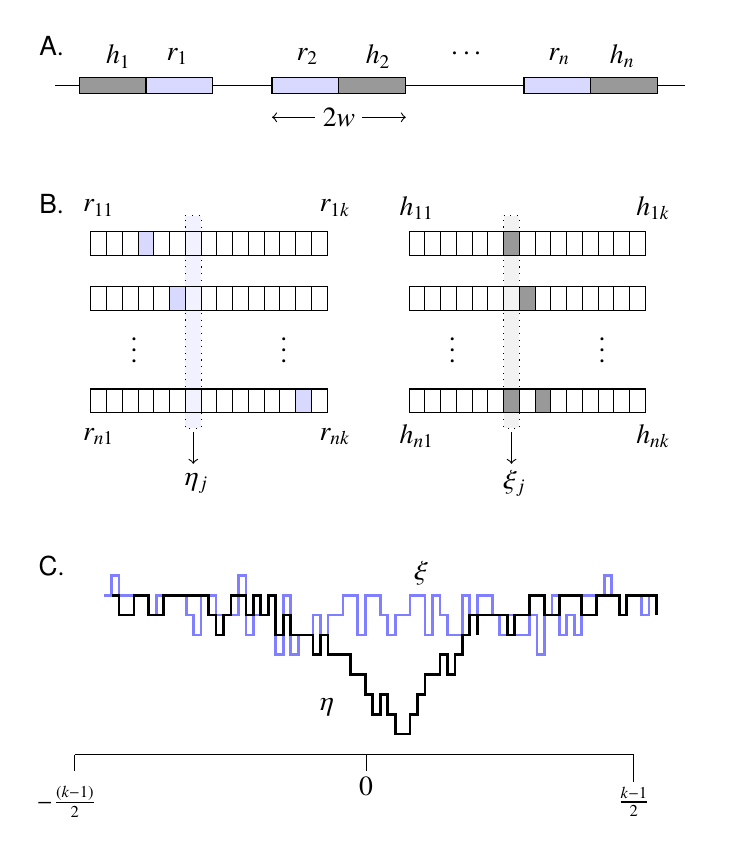
\begin{tikzpicture}
 %
 %% hotspot + reference regions
 %
 \node at (-0.05,0.5) {\textsf{A}.};
 \draw (0,0) -- (8,0);
 \draw[fill=black!40] (0.3,-0.1) -- (1.15,-0.1) -- (1.15,0.1) -- (0.3,0.1) -- cycle;
 \draw[fill=blue!15] (1.15,-0.1) -- (2,-0.1) -- (2,0.1) -- (1.15,0.1) -- cycle;
 \draw[fill=blue!15] (5.95,-0.1) -- (6.8,-0.1) -- (6.8,0.1) -- (5.95,0.1) -- cycle;
 \draw[fill=black!40] (6.8,-0.1) -- (7.65,-0.1) -- (7.65,0.1) -- (6.8,0.1) -- cycle;
 \draw[fill=blue!15] (2.75,-0.1) -- (3.6,-0.1) -- (3.6,0.1) -- (2.75,0.1) -- cycle;
 \draw[fill=black!40] (3.6,-0.1) -- (4.45,-0.1) -- (4.45,0.1) -- (3.6,0.1) -- cycle;
 % labels
 \node at (0.8,0.37) {$h_1$};
 \node at (1.55,0.37)  {$r_1$};
 \node at (4.1,0.37)  {$h_2$};
 \node at (3.2,0.37) {$r_2$};
 \node at (5.25,0.37)  {$\cdots$};
 \node at (6.4,0.37)  {$r_n$};
 \node at (7.2,0.37)  {$h_n$};
 %
 \draw[<-] (2.75,-0.4) -- (3.3,-0.4);
 \draw[->] (3.89,-0.4) -- (4.45,-0.4);
 \node at (3.6,-0.4) {$2w$};
 %
 %% The r_{ij} matrix
 %
 \node at (-0.05,-1.5) {\textsf{B}.};
 \begin{scope}[yshift=-10pt]
  % vertical rectangle
  \draw[dotted, fill=blue!5] (1.65,-1.3) -- (1.85,-1.3) -- (1.85, -4) -- (1.65, -4) -- cycle;
  % rows
  \draw (0.45, -1.5) -- (3.45, -1.5) -- (3.45, -1.8) -- (0.45, -1.8) -- cycle;
  \foreach \x in {0.45, 0.65,..., 3.35} {\draw (\x, -1.5) -- (\x, -1.8);}
  \draw[fill=blue!15] (1.05, -1.5) -- (1.25, -1.5) -- (1.25, -1.8) -- (1.05, -1.8) -- cycle;
  %\draw[fill=blue!15] (2.05, -1.5) -- (2.25, -1.5) -- (2.25, -1.8) -- (2.05, -1.8) -- cycle;
  \draw (0.45, -2.2) -- (3.45, -2.2) -- (3.45, -2.5) -- (0.45, -2.5) -- cycle;
  \foreach \x in {0.45, 0.65,..., 3.35} {\draw (\x, -2.2) -- (\x, -2.5);}
  \draw[fill=blue!15] (1.45, -2.2) -- (1.65, -2.2) -- (1.65, -2.5) -- (1.45, -2.5) -- cycle;
  \node at (2.9, -2.9) {$\vdots$};
  \node at (1, -2.9) {$\vdots$};
  \draw (0.45, -3.5) -- (3.45, -3.5) -- (3.45, -3.8) -- (0.45, -3.8) -- cycle;
  \foreach \x in {0.45, 0.65,..., 3.35} {\draw (\x, -3.5) -- (\x, -3.8);}
  \draw[fill=blue!15] (3.05, -3.5) -- (3.25, -3.5) -- (3.25, -3.8) -- (3.05, -3.8) -- cycle;
  \draw[->] (1.75, -4.05) -- (1.75, -4.45);
  % labels
  \node at (1.79, -4.7) {$\eta_j$};
  \node at (0.55, -1.2) {$r_{11}$};
  \node at (3.55, -1.2) {$r_{1k}$};
  \node at (0.55, -4.1) {$r_{n1}$};
  \node at (3.55, -4.1) {$r_{nk}$};
  % border
  %\draw[dashed] (0.3,-1.3) -- (3.6,-1.3) -- (3.6, -4) -- (0.3, -4) -- cycle;
 \end{scope}
 %
 %% The h_{ij} matrix
 %
 \begin{scope}[yshift=-10pt, xshift=115pt]
  % vertical rectangle
  \draw[dotted, fill=gray!10] (1.65,-1.3) -- (1.85,-1.3) -- (1.85, -4) -- (1.65, -4) -- cycle;
  % rows
  \draw (0.45, -1.5) -- (3.45, -1.5) -- (3.45, -1.8) -- (0.45, -1.8) -- cycle;
  \foreach \x in {0.45, 0.65,..., 3.35} {\draw (\x, -1.5) -- (\x, -1.8);}
  \draw[fill=black!40] (1.65, -1.5) -- (1.85, -1.5) -- (1.85, -1.8) -- (1.65, -1.8) -- cycle;
  \draw (0.45, -2.2) -- (3.45, -2.2) -- (3.45, -2.5) -- (0.45, -2.5) -- cycle;
  \foreach \x in {0.45, 0.65,..., 3.35} {\draw (\x, -2.2) -- (\x, -2.5);}
  \draw[fill=black!40] (1.85, -2.2) -- (2.05, -2.2) -- (2.05, -2.5) -- (1.85, -2.5) -- cycle;
  \node at (2.9, -2.9) {$\vdots$};
  \node at (1, -2.9) {$\vdots$};
  \draw (0.45, -3.5) -- (3.45, -3.5) -- (3.45, -3.8) -- (0.45, -3.8) -- cycle;
  \foreach \x in {0.45, 0.65,..., 3.35} {\draw (\x, -3.5) -- (\x, -3.8);}
  \draw[fill=black!40] (1.65, -3.5) -- (1.85, -3.5) -- (1.85, -3.8) -- (1.65, -3.8) -- cycle;
  \draw[fill=black!40] (2.05, -3.5) -- (2.25, -3.5) -- (2.25, -3.8) -- (2.05, -3.8) -- cycle;
  \draw[->] (1.75, -4.05) -- (1.75, -4.45);
  % labels
  \node at (1.79, -4.7) {$\xi_j$};
  \node at (0.55, -1.2) {$h_{11}$};
  \node at (3.55, -1.2) {$h_{1k}$};
  \node at (0.55, -4.1) {$h_{n1}$};
  \node at (3.55, -4.1) {$h_{nk}$};
 \end{scope}
 %
 %% The ``sum'' of all histograms
 %
 \node at (-0.05,-6.1) {\textsf{C}.};
 \begin{scope}[xshift=-30pt, yshift=20pt]
  \begin{axis}[
    width=10cm, height=4cm,
    at={(0.08\linewidth,-260pt)},
    hide x axis,
    hide y axis,
    mark size = 0pt
    ]
  \addplot+[const plot, draw=blue!50, line width=1pt]%
   coordinates {
    (-10,0) (-9,1) (-8,-0) (-7,-0) (-6,0)  
    (-5,0) (-4,-1) (-3,-0) (-2,-0) (-1,0)  (0,0)
    (1,-1) (2,-2) (3,-0) (4,-0) (5,-1) 
    (6,-1) (7,-1) (8,1) (9,-2) (10,-1) 
    (11,-1) (12,-0) (13,-3) (14,0) (15,-3) 
    (16,-2) (17,-2) (18,-1) (19,-2) (20,-1) 
    (21,-1) (22,0) (23, 0) (24,-2) (25,0) 
    (26,0) (27,-1) (28,-2) (29,-1) (30,-1)
    (31,0) (32,0) (33,-2) (34,0) (35,-1)
    (36,-2) (37,-2) (38,0) (39,-1) (40,-1)
    (40,-0) (41,-0) (42,-1) (43,-2) (44,-1) 
    (45,-2) (46,-2) (47,-1) (48,-3) (49,-1) 
    (50,0) (51,-2) (52,-1) (53,-2) (54,0)
    (55,0) (56,0) (57,1) (58,0) (59,-1)
    (60,0) (61,0) (62,-1) (63,0) (64,-1)
 };
  \addplot+[const plot, draw=black, line width=1pt]%
   coordinates {
     (-9,0) (-8,-1) (-7,-1) (-6,0) (-5,0) 
    (-4,-1) (-3,-1) (-2,-0) (-1,-0) (0,0) 
    (1,0) (2,0) (3,0) (4,-1) (5,-2) 
    (6,-1) (7,0) (8,0) (9,-1) (10,0) 
    (11,-1) (12,-0) (13,-2) (14,-1) (15,-2) 
    (16,-2) (17,-2) (18,-3) (19,-2) (20,-3) 
    (21,-3) (22,-3) (23, -4) (24,-4) (25,-5) 
    (26,-6) (27,-5) (28,-6) (29,-7) (30,-7)
    (31,-6) (32,-5) (33,-4) (34,-4) (35,-3)
    (36,-4) (37,-3) (38,-2) (39,-1) (40,-2)
    (40,-1) (41,-1) (42,-1) (43,-1) (44,-2) 
    (45,-1) (46,-1) (47,0) (48,0) (49,-1) 
    (50,-1) (51,0) (52,0) (53,0) (54,-1) 
    (55,-1) (56,0) (57,0) (58,0) (59,-1)
    (60,0) (61,0) (62,0) (63,0) (64,-1)
  };
 \end{axis}
 \node at (5.7, -6.9) {$\xi$};
 \node at (4.5,-8.6) {$\eta$};

 \draw (1.3,-9.2) -- (8.4,-9.2);
  
  \draw (1.3, -9.2) -- (1.3, -9.4);
  \draw (5, -9.2) -- (5, -9.4);
  \draw (8.4, -9.2) -- (8.4, -9.54);
  
  \node at (5, -9.6) {0};
  \node at (1.2, -9.8) {\small $-\frac{(k-1)}{2}$};
  \node at (8.4, -9.8) {\small $\frac{k-1}{2}$};
 \end{scope}
\end{tikzpicture}
 \label{fig:methodscheme}
 \caption{A: Input data segments $h_1, \ldots, h_n$ containing the occurence of a string $\mathcal S$ and reference segments $r_1, \ldots, r_n$. B: $r_{ij}$ and $h_{ij}$ matrizes of counts for a particular realization of the random variables $\eta_{ij}$, $\xi_{ij}$. C: Profile distribution for the occurence of $\mathcal S$ along a hotspost and a reference region.}
\end{figure}


The basic question we like to address is wether the distribution profile of the string $\mathcal S$ is significatively different along a typical hotspot region and a reference region. This may be assessed  by considering the following $2\times k$ contingency table
\[
  \begin{bmatrix}
  \xi_1 & \xi_2 & \ldots & \xi_k\\
  \eta_1 & \eta_2 & \ldots & \eta_k
  \end{bmatrix},
\]
obtained by merging the two vectors of counts $\xi_j$ and $\eta_j$. Provided the number of counts in each of the cells of this table is sufficiently large, the significance of a differential profile can be determined by using Pearson's $X^2$ statistic, which is distributed according to a $\chi^2$ density with $k-1$ degrees of freedom. Other alternatives for the large sample case exist, see for instance~\cite{RC}, but we do not pursue this further here.  It is well known that this procedure can give a poor approximation when several cells present low counts (smaller than 10). This may be the case in the current setting when analysing the profile distribution of longer strings with $\ell \geq 10$ or even smaller but rarely occuring strings. In these situations the significance for a differential profile is more appropriately determined by using Fisher's exact test, see for instance~\cite{A}. The computations necessary to derive a $p$-value are not feasible because of the large number of contingency tables that have to be considered as a reference set when $k$ is large. The significance may however be approximately computed by considering a permutation test using the method in \cite{P}. We found that R's implementation via \texttt{fisher.test} takes only few secconds for relatively large tables with $k=1000$.


We provide examples for the two scenarios just mentioned by considering strings formed by a single base and strings defined by longer motivs with $\ell = 15$. The former provides an example where the $X^2$ statistic is a appropriate and the latter one that is amenable to the analysis with Fisher's exact test.

\section{Results}
Put the plots and the $p$-values.

\section{Discussion}
Mention that the results are surprising and important from the perspective of  the virus insertion problem. Then talk very briefly about the scope of this method: what kind of problems can we consider.

\bibliographystyle{natbib}
\scriptsize{
   \bibliography{rich}
\normalsize
}
\end{document}
